\centering

  \begin{subfigure}[c]{0.3\textwidth}
    \centering
    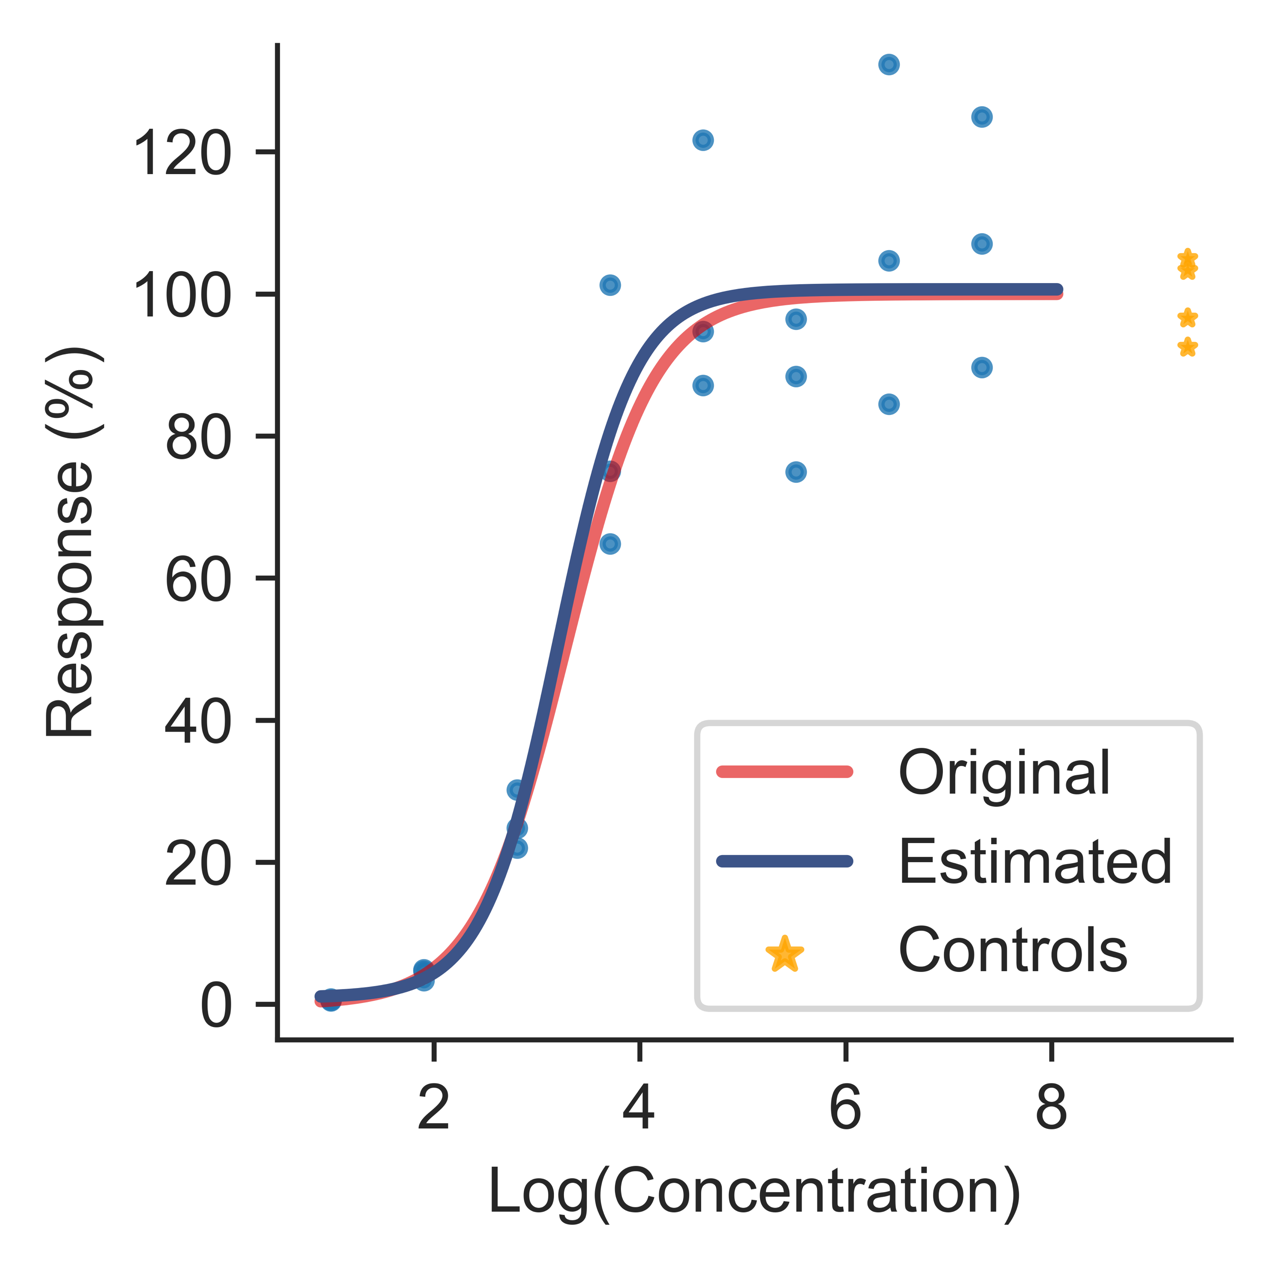
\includegraphics[width=0.9\textwidth]{figures/plate_layout_rand_02.npy_compound_1-right-half.png}
    \caption{$R^2=0.91$, $IC_{50}=61.92$}
    \label{fig:dr-borer-comp1}
  \end{subfigure}
  \hfill
  \begin{subfigure}[c]{0.3\textwidth}
    \centering
    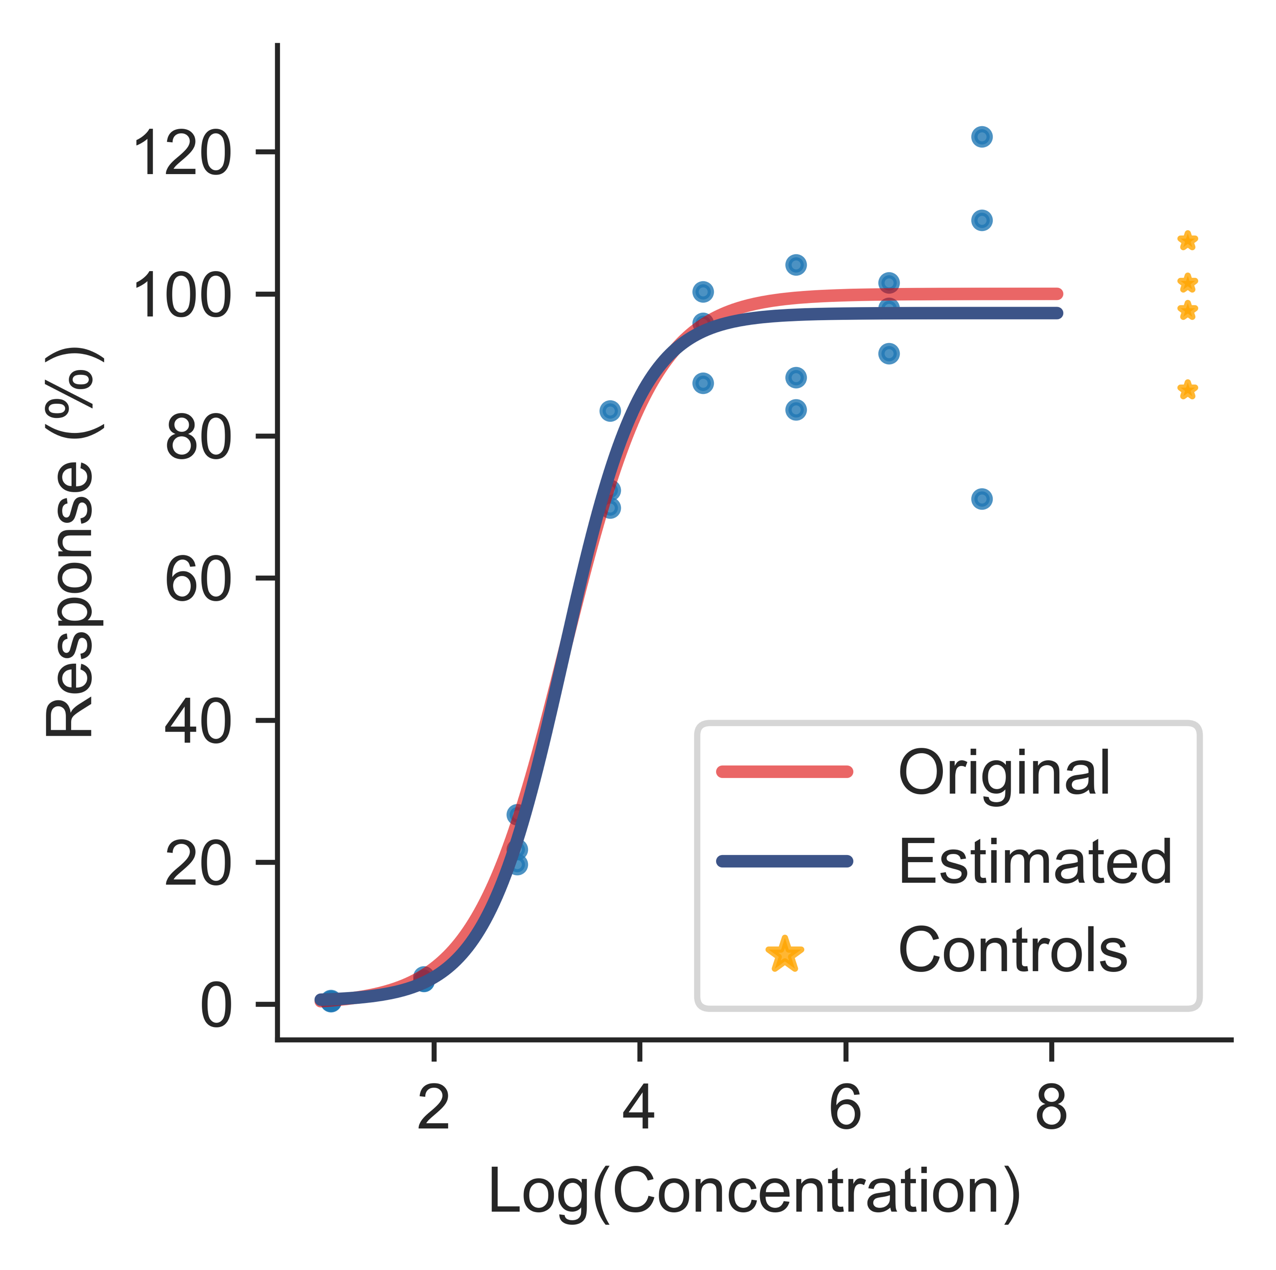
\includegraphics[width=0.9\textwidth]{figures/plate_layout_20-12-8-3_01.npy_compound_1-right-half.png}
    \caption{$R^2=0.95$, $IC_{50}=55.48$}
    \label{fig:dr-rand-comp1}
  \end{subfigure}
  \hfill
    \begin{subfigure}[c]{0.3\textwidth}
    \centering
    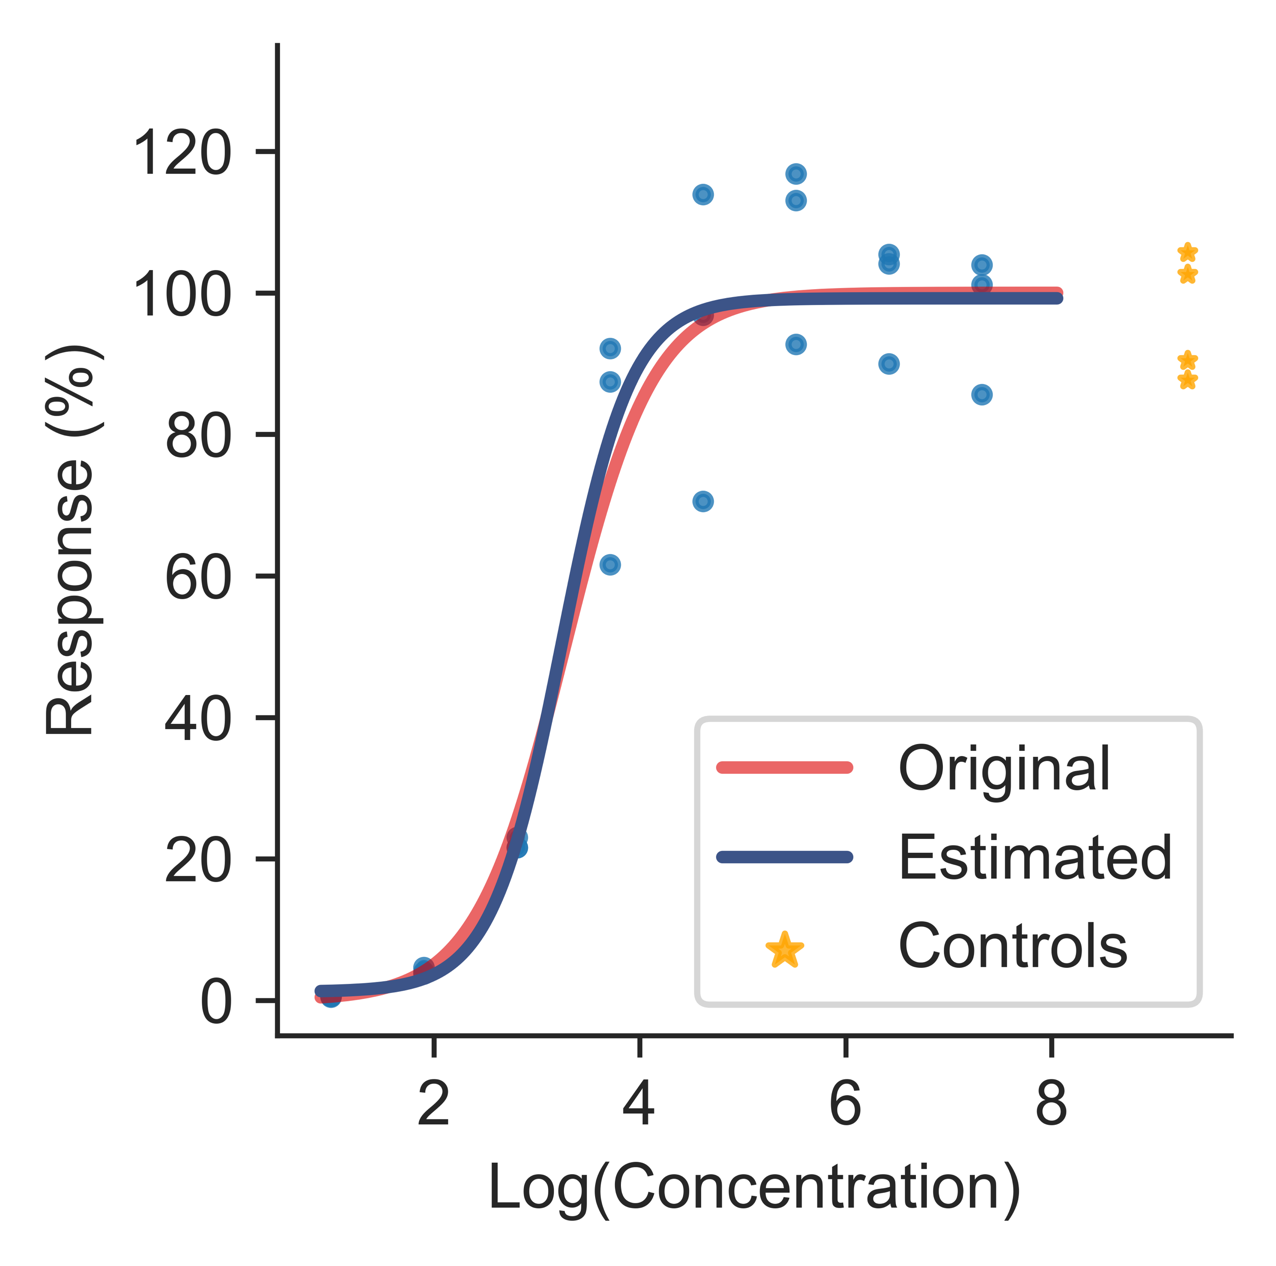
\includegraphics[width=0.9\textwidth]{figures/plate_layout_40-12-8-3_01.npy_compound_1-right-half.png}
    \caption{$R^2=0.95$, $IC_{50}=57.66$}
    \label{fig:dr-plaid-comp1}
  \end{subfigure}

  \caption{An example of dose response curves for simulated experiments
    using 8~doses with 3~replicates (blue dots), 4~negative controls
    (yellow stars), and strong bowl-shaped plate effects on layouts constructed (a) randomly, (b) with PLAID and (c) with COMPD. The expected $IC_{50} = 53.43$. On the caption
    below each plot we show the obtained $R^2$ and $IC_{50}$ values.}
  \label{fig:dose-response-curves-paper} 








%%% Local Variables: 
%%% mode: latex
%%% TeX-master: "../supplement.tex"
%%% End: 